\section{Hybrid positioning and Kalman filter}

The absolute positioning method is quit accurate but still suffers from noise. On the other hand relative positioning has a lot of uncertainty, because of the physical interference. By combing these two positioning methods we can get more precise location based on sensor measurements from absolute and prediction from the relative positions. This combination is called hybrid positioning. One of the methods achieving hybrid position is with Kalman filter.

The Kalman filter was made by Rudolf E. Kalman and developed for the Apollo 11 mission\footnote{\cite{Grewal2010}} to the moon to track the location of the space shuttle. This method is still used because it does not require a lot of processing power or memory space. The reasoning is that the method does not need to save any data apart from the model of movement and the previous position. The filter predicts a position based on the model and previous positions. After the prediction, the real position is being measured and the filter corrects its prediction by multiplying both Gaussian distributions thus producing a more precise prediction of position.

\begin{figure}[H]
	\centering
	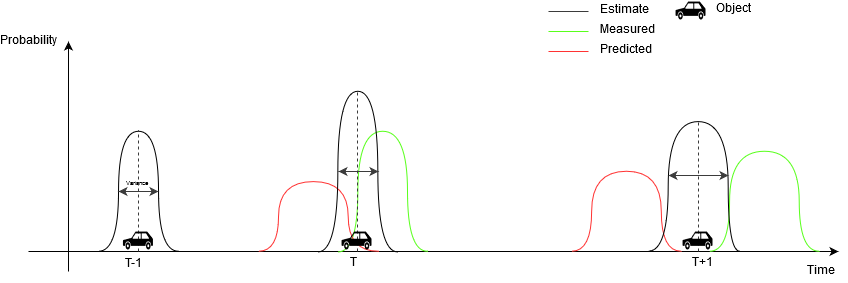
\includegraphics[width=0.7\linewidth]{positioning/positioning/DiagramKalman}
	\caption{The workings of the Kalman filter.}
	\label{fig:Kalmanfilter}
\end{figure}

In figure \ref{fig:Kalmanfilter} we see how the filter is working. There are two cases in it. First one is when time is (T-1) and (T). In this first case we can see that the filter goes closer to the measured distribution, because it is more reliable. Also from the graph we can see the power of hybrid position: The probability is estimating the position correct is higher than absolute and relative positioning. The second case is when time is (T) and (T+1). In this case the measurements contain a lot more noise. Then the estimation is moving further from the measured distribution because of the lower probability.